\documentclass[11pt, oneside]{article}   	% use "amsart" instead of "article" for AMSLaTeX format
\usepackage{geometry}                		% See geometry.pdf to learn the layout options. There are lots.
\geometry{letterpaper}                   		% ... or a4paper or a5paper or ... 
%\geometry{landscape}                		% Activate for for rotated page geometry
%\usepackage[parfill]{parskip}    		% Activate to begin paragraphs with an empty line rather than an indent
\usepackage{graphicx}				% Use pdf, png, jpg, or eps� with pdflatex; use eps in DVI mode
								% TeX will automatically convert eps --> pdf in pdflatex		
\usepackage{amssymb}

\title{Whats up with Mercury?}
\author{Team Mercury}
%\date{}							% Activate to display a given date or no date

\begin{document}
\maketitle

\section{BIG QUESTIONS:}
\begin{itemize}
	\item What is the large scale internal structure (e.g. Inner Core Radius, does a high density layer exist )?
	\item Alternative ways to power the dynamo (e.g. Precession Drive Dynamo from tidal resonance versus Double diffusive convection)
\end{itemize}

\subsection{Internal Structure}
What is the first order radial structure?
\begin{itemize}
	\item What is the depth of the inner core? 
	\item What can we say about the proposed high density layer at the base of the mantle?
	\item Can we use 1-D parameterized models of convection and dynamo energetics to connect 	
		these two ideas and better constrain them?
	\item How do these two tradeoff?
\end{itemize}

\begin{figure}[htbp]
\begin{center}
	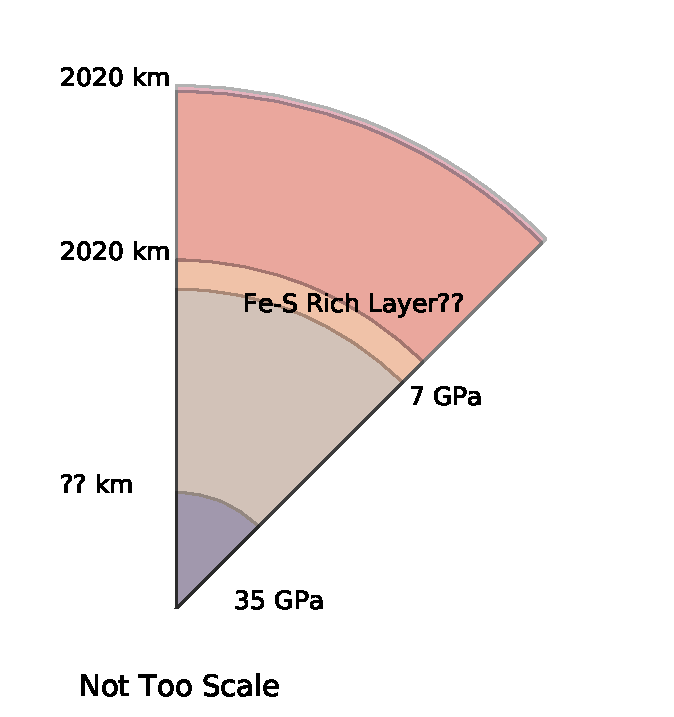
\includegraphics[scale=0.8]{Mercury_Schematic.pdf}
\caption{default}
\label{default}
\end{center}
\end{figure}


\subsubsection{Known Constraints:}
\begin{itemize}
	\item Radius of Mercury: 2440 km 
		\item CMB: 2020 km \cite{hauck2013curious}
		\item Elastic Thickness: 25-30 km \cite{nimmo2004depth}
		\item Crustal Thickness: 140 km \cite{nimmo2004depth}
\end{itemize}

\subsection{Powering the Dynamo}
\begin{itemize}
	\item Convection Driven
	\item Precession Driven 
\end{itemize}

\bibliographystyle{plain}
\bibliography{mercury.bib}

\end{document}  
